\documentclass[notes]{subfiles}
\begin{document}
	\addcontentsline{toc}{section}{How Can Data Be Misrepresented?}
	\refstepcounter{section}
	\fancyhead[RO,LE]{\bfseries \large \nameref{misrepresent}} 
	\fancyhead[LO,RE]{\bfseries \currentname}
	\fancyfoot[C]{{}}
	\fancyfoot[RO,LE]{\large \thepage}	%Footer on Right \thepage is pagenumber
	\fancyfoot[LO,RE]{\large Unit 1}

\section*{How Can Data Be Misrepresented?}\label{misrepresent}
	\subsection*{Qualitative Data}
		It is not uncommon for data to be used to misinform or mislead.  We'll explore some ways graphs can be used to misrepresent data and some ways to identify when that happens.%
		
		\begin{ex}
			The seasonally adjusted annual rate for new single-family houses sold in the United States (in thousands) between January 2020 and April 2020 is shown in the bar graph below.%
			\begin{center}
				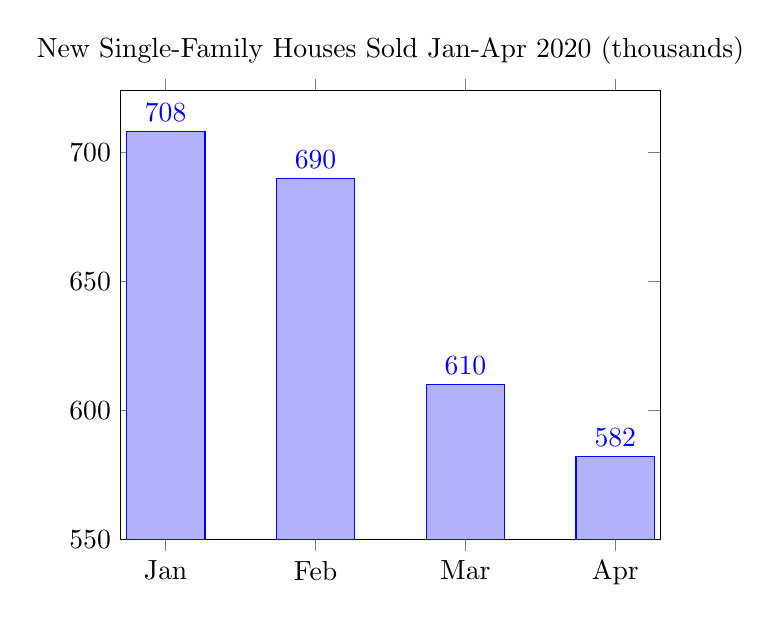
\begin{tikzpicture}
				    \begin{axis}[
				        title = New Single-Family Houses Sold Jan-Apr 2020 (thousands),
				        ybar,
				        nodes near coords,
				        bar width = 1cm,
				        symbolic x coords = {Jan, Feb, Mar, Apr},
				        xtick = {Jan, Feb, Mar, Apr},
				        ymin = 550
				    ]
				    \addplot coordinates {(Jan, 708) (Feb, 690) (Mar, 610) (Apr, 582)};
				    \end{axis}
				\end{tikzpicture}
			\end{center}
			Discuss why this bar graph might be misleading.%
		\end{ex}
			\vs{1}
			\newpage
			
		\begin{ex}
			The same data from the previous example is graphed again below.%
			\begin{center}
				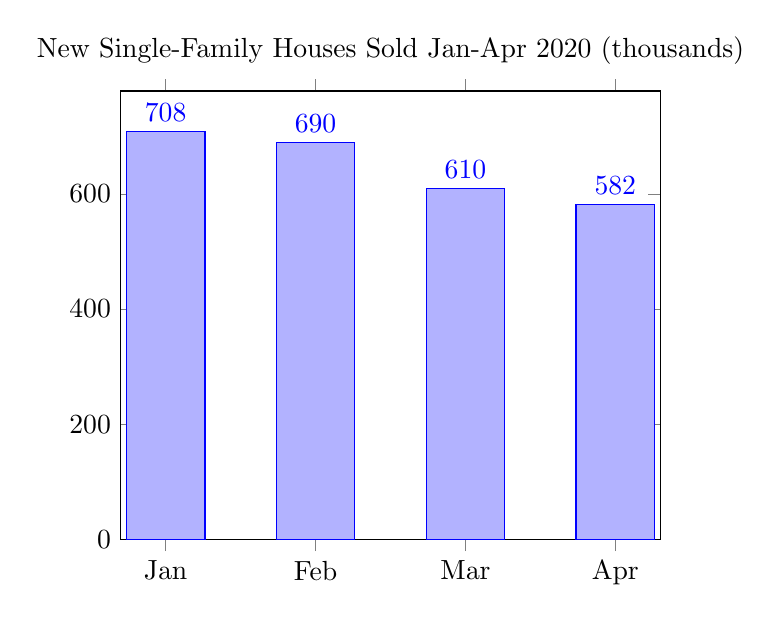
\begin{tikzpicture}
				    \begin{axis}[
				        title = New Single-Family Houses Sold Jan-Apr 2020 (thousands),
				        ybar,
				        nodes near coords,
				        bar width = 1cm,
				        symbolic x coords = {Jan, Feb, Mar, Apr},
				        xtick = {Jan, Feb, Mar, Apr},
				        ymin = 0
				    ]
				    \addplot coordinates {(Jan, 708) (Feb, 690) (Mar, 610) (Apr, 582)};
				    \end{axis}
				\end{tikzpicture}
			\end{center}
			What is different about this graph than the previous one?  In what ways might it be a better representation of the data?
		\end{ex}
			\vs{1}
			\newpage
			
		\begin{rmk}[Common Ways to Mislead Using Graphs]
			$ $\\[5pt]
			\tabitem Adjusting $y-$axis\\[15pt]
			\tabitem Using the wrong graphic\\[15pt]
			\tabitem Poor scaling or labeling\\[15pt]
			\tabitem Cherry picking
		\end{rmk}
		
		\begin{ex}
			Why would a pie chart be inappropriate for displaying the new home sales data?%
		\end{ex}
			\vs{1}
			
		\begin{ex}
			Describe why the graph below might be considered misleading.%
			\begin{flushleft}
				
\includegraphics[scale=.75]{../assets/pictograph_scaled.png}
			\end{flushleft}
		\end{ex}
			\vs{1}
			\newpage
			
		\begin{ex}
			Discuss your thoughts about the graphic below with one or two people near you.  What do you notice?  What do you believe is missing?%
			\begin{flushleft}
				\includegraphics[scale=.2]{../assets/fl_gun_deaths.jpg}
			\end{flushleft}
		\end{ex}
			
		\begin{ex}
			The graph below shows the total amount of debt (in trillions) held by the US government between January and July 2020.%
			\begin{center}
				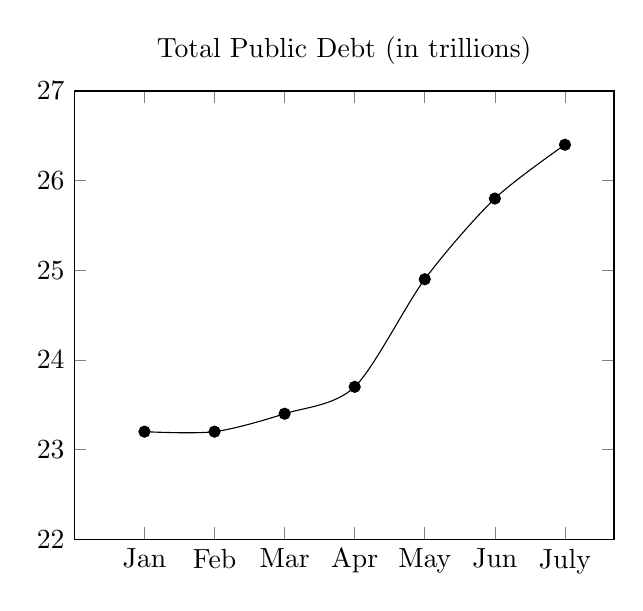
\begin{tikzpicture}
				    \begin{axis}[
				        title = Total Public Debt (in trillions),
				        xmin =0,
				        ymin = 22, ymax = 27,
				        xtick = {1,2,3,4,5,6,7},
				        xticklabels = {Jan,Feb,Mar,Apr,May,Jun,July}
				    ]
				        \addplot[smooth, mark = *] plot coordinates {(1, 23.2) (2, 23.2) (3, 23.4) (4, 23.7) (5, 24.9) (6, 25.8) (7, 26.4)};
				    
				    \end{axis}
				\end{tikzpicture}
			\end{center}
			Do you think that the graph gives an accurate picture of the rise of national debt?  Why or why not?%
		\end{ex}
\clearpage
\end{document}